\documentclass[12pt,letterpaper]{article}
\usepackage[top=1in,bottom=1in,left=1in,right=1in]{geometry}
\usepackage{amsmath,amssymb}
\usepackage{tikz}
\usetikzlibrary{decorations.pathreplacing}
\usepackage{ulem}
\usepackage{enumitem}

\setlength{\parindent}{0pt}
\setlength{\parskip}{4pt}

\begin{document}

% ── Cover Page ────────────────────────────────────────────────────────────────
\begin{center}
  {\Large\textbf{ECE 332 Fall 2025}}\\[8pt]
  {\Large\textbf{Exam 1}}\\[8pt]
  (100 pts total)\\[8pt]
  November 6, 2025
\end{center}

\vspace{14pt}

\uline{Allowed}: Calculator approved for the FE exam and a 2-sided page of notes.\\
\hspace*{58pt}\uline{Not allowed}: Any other devices or materials.

\vspace{14pt}

Use the approximations
\[
  \epsilon_0 \approx \frac{1}{36\pi} \times 10^{-9}\ \text{F/m}, \qquad
  \mu_0 = 4\pi \times 10^{-7}\ \text{H/m}, \qquad
  \eta_0 \approx 120\pi\ \Omega
\]
in your calculations.

\vspace{10pt}
\uline{Useful Facts}:\\[4pt]
``Special'' right triangles:

\vspace{8pt}
\begin{center}
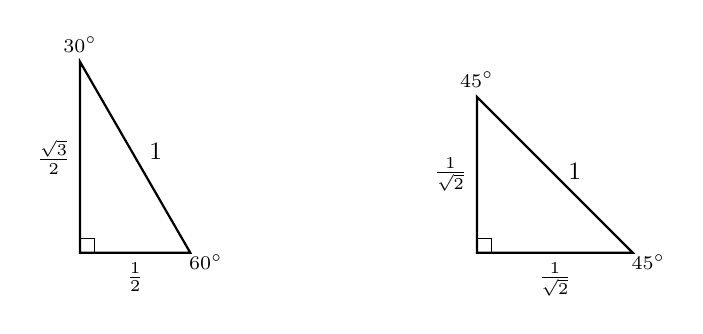
\begin{tikzpicture}[scale=2.8, font=\small]
  % --- 30-60-90 triangle ---
  % Right angle at bottom-left, short leg (1/2) along bottom, long leg (sqrt3/2) along left
  \coordinate (A) at (0,0);       % right angle
  \coordinate (B) at (0.5,0);     % 60 degree angle
  \coordinate (C) at (0,0.866);   % 30 degree angle
  \draw[thick] (A) -- (B) -- (C) -- cycle;
  \draw (0.065,0) -- (0.065,0.065) -- (0,0.065);
  \node[below] at (0.25,0)       {$\tfrac{1}{2}$};
  \node[left]  at (0,0.433)      {$\tfrac{\sqrt{3}}{2}$};
  \node[right] at (0.27,0.46)    {$1$};
  \node[above, font=\scriptsize] at (C) {$30^\circ$};
  \node[below right, font=\scriptsize, xshift=-4pt, yshift=3pt] at (B) {$60^\circ$};

  % --- 45-45-90 triangle ---
  \begin{scope}[xshift=1.8cm]
    \coordinate (A2) at (0,0);
    \coordinate (B2) at (0.707,0);
    \coordinate (C2) at (0,0.707);
    \draw[thick] (A2) -- (B2) -- (C2) -- cycle;
    \draw (0.065,0) -- (0.065,0.065) -- (0,0.065);
    \node[below] at (0.354,0)     {$\tfrac{1}{\sqrt{2}}$};
    \node[left]  at (0,0.354)     {$\tfrac{1}{\sqrt{2}}$};
    \node[right] at (0.37,0.37)   {$1$};
    \node[above, font=\scriptsize] at (C2) {$45^\circ$};
    \node[below right, font=\scriptsize, xshift=-4pt, yshift=3pt] at (B2) {$45^\circ$};
  \end{scope}
\end{tikzpicture}
\end{center}

\vspace{10pt}

The area of a triangle is $A = \frac{1}{2}bh$, where $b$ is the length of the ``base'' and $h$ is the ``height.''

\begin{center}
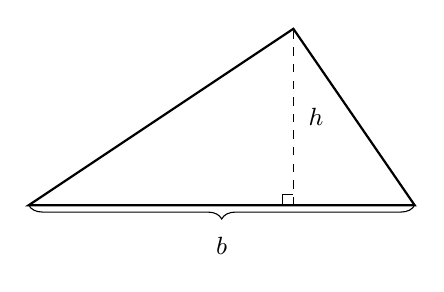
\begin{tikzpicture}[scale=1.4]
  \draw[thick] (0,0) -- (3.5,0) -- (2.4,1.6) -- cycle;
  \draw[dashed] (2.4,0) -- (2.4,1.6);
  \draw (2.3,0) -- (2.3,0.1) -- (2.4,0.1);
  \node[right, font=\small] at (2.45,0.8) {$h$};
  \draw[decorate, decoration={brace, amplitude=5pt, mirror}]
    (0,0) -- (3.5,0) node[midway, below=8pt, font=\small] {$b$};
\end{tikzpicture}
\end{center}

\newpage

% ── Question 1 ────────────────────────────────────────────────────────────────
\textbf{1.}\ (20 points total) Suppose an equilateral triangular conducting loop of $N$ turns
with sides of length $a$ is located in the $y$-$z$ plane with normal $d\mathbf{s} = \hat{x}\,ds$,
as shown below,

\begin{center}
\begin{tikzpicture}[scale=1.4]
  % Axes: y right, z up, x diagonal toward lower-left
  \draw[->] (0,0) -- (2.5,0)   node[right] {$y$};
  \draw[->] (0,0) -- (0,2.5)   node[above] {$z$};
  \draw[->] (0,0) -- (-0.9,-0.65) node[below left] {$x$};
  % Equilateral triangle in y-z plane (roughly centered at (1.4, 1.6))
  % Side ~ 0.6 units
  \coordinate (T1) at (1.1, 1.35);
  \coordinate (T2) at (1.7, 1.35);
  \coordinate (T3) at (1.4, 1.87);
  \draw[thick] (T1) -- (T2) -- (T3) -- cycle;
  \node[below, font=\small] at (1.4, 1.32) {$a$};
  \node[right, font=\small] at (1.72, 1.6)  {$a$};
  \node[left,  font=\small] at (1.08, 1.6)  {$a$};
\end{tikzpicture}
\end{center}

in a magnetic field
\[
  \mathbf{B}(t) = B_0(-2\hat{x} + 3\hat{y})\sin(\omega t).
\]

\begin{enumerate}[label=(\alph*), leftmargin=2.5cm]

  \item Find a formula for the magnetic flux through one turn of the loop.
        \hfill(6 points)
  \vspace{5.5cm}

  \item Find a formula for the emf induced in the loop at time $t$.
        \hfill(6 points)
  \vspace{5.5cm}

  \item Determine the current flowing through a $1\,\mathrm{k\Omega}$ resistor incorporated
        in the loop when $N = 10$, $a = 8\,\mathrm{cm}$, $B_0 = 0.02\,\mathrm{T}$,
        $\omega = 2\,\mathrm{MHz}$, and $\omega t = \pi/4$, assuming that the resistance
        of the loop material is negligible.
        \hfill(8 points)
  \vspace{6cm}

\end{enumerate}

\newpage

% ── Question 2 ────────────────────────────────────────────────────────────────
\textbf{2.}\ A straight conducting wire of length $a = 15\,\mathrm{cm}$ lying along the
$\hat{y}$ direction moves with velocity $\mathbf{u} = 12\hat{x}\,\mathrm{cm/s}$ in a
magnetic field
\[
  \mathbf{B} = (0.1\hat{x} - 0.05\hat{z})\ \mathrm{T}.
\]
Find the emf between the two ends of the wire. \hfill(12 points)

\vspace{13cm}

% ── Question 3 ────────────────────────────────────────────────────────────────
\textbf{3.}\ Suppose a total conduction current $I_c = 2\sin(\omega t)\ \mu\mathrm{A}$ flows
through a column of distilled water with cross-sectional area $A$ in a glass tube.
Distilled water has conductivity $\sigma \approx 10^{-4}\,\mathrm{S/m}$ and relative
permittivity $\epsilon_r \approx 26\pi$ and the current flowing through the glass is
negligible compared to the current flowing through the water. (12 points total)

\begin{enumerate}[label=(\alph*), leftmargin=2.5cm]

  \item Use the relationship between the conduction current, the current density, the
        cross-sectional area, and Ohm's law to determine the electric field intensity
        $E$ at a cross-section of the water.
        \hfill(6 points)
  \vspace{5.5cm}

  \item Determine the displacement current $I_d$ through the cross-section when the
        angular frequency of $I_c$ is $\omega = 10^9\,\mathrm{rad\,s^{-1}}$ and
        $\omega t = \pi/3$.
        \hfill(6 points)
  \vspace{5.5cm}

\end{enumerate}

\newpage

% ── Question 4 ────────────────────────────────────────────────────────────────
\textbf{4.}\ Distilled water has a conductivity $\sigma \approx 10^{-4}\,\mathrm{S/m}$
and $\epsilon_r \approx 26\pi$. (10 points total)

\begin{enumerate}[label=(\alph*), leftmargin=2.5cm]

  \item Find the relaxation time constant for distilled water.
        \hfill(5 points)
  \vspace{7cm}

  \item How long does it take for an excess charge density in distilled water to decay
        to $e^{-3}$ times its initial value?
        \hfill(5 points)
  \vspace{7cm}

\end{enumerate}

\newpage

% ── Question 5 ────────────────────────────────────────────────────────────────
\textbf{5.}\ (30 points total) Suppose the electric field intensity of an EM wave in a
nonconducting, source-free medium with $\epsilon_r = 6$ and $\mu_r = 1$ is
\[
  \mathbf{E}(z,t) = 4\cos\!\left((6\pi \times 10^8\ \mathrm{rad/s})\,t - kz
    - \frac{\pi}{6}\right)\hat{y}\ \mathrm{V/m}.
\]

\begin{enumerate}[label=(\alph*), leftmargin=2.5cm]

  \item Determine the angular frequency $\omega$, the wavenumber $k$, the wavelength
        $\lambda$, and the intrinsic impedance $\eta$.
        \hfill(10 points)
  \vspace{8cm}

  \item Find $\tilde{\mathbf{E}}(z)$.
        \hfill(5 points)
  \vspace{4.5cm}

  \item Find $\tilde{\mathbf{H}}(z)$.
        \hfill(5 points)
  \vspace{4.5cm}

  \item Determine the magnetic field intensity $\mathbf{H}(z,t)$.
        \hfill(5 points)
  \vspace{4.5cm}

  \item Determine the average power density that the EM wave carries.
        \hfill(5 points)
  \vspace{4cm}

\end{enumerate}

\newpage

% ── Question 6 ────────────────────────────────────────────────────────────────
\textbf{6.}\ Consider a $\tfrac{2}{\pi}\,\mathrm{GHz}$ EM wave traveling in distilled
water, where $\sigma \approx 10^{-4}\,\mathrm{S/m}$, $\epsilon_r \approx 26\pi$, and
$\mu_r = 1$. The wave travels downward into the water, where the $+z$ direction is down
and $z = 0$ is just below the surface. The amplitude of the electric field at the surface
is $4\,\mathrm{V/m}$. (16 points total)

\begin{enumerate}[label=(\alph*), leftmargin=2.5cm]

  \item Find $\epsilon''/\epsilon'$.
        \hfill(6 points)
  \vspace{7cm}

  \item What type of medium is distilled water at this frequency? Justify your answer.
        \hfill(5 points)
  \vspace{6cm}

  \item Find the skin depth for distilled water at this frequency.
        \hfill(5 points)
  \vspace{6cm}

\end{enumerate}

\end{document}
